\documentclass[compress]{beamer}
\usepackage[utf8]{inputenc}
\usepackage{hyperref}

\usepackage{tikz}
\usetikzlibrary{graphs, quotes, arrows.meta, matrix}

\usetheme{default}
\usecolortheme{Nord}
\setbeamertemplate{navigation symbols}{}

\title{Stringhe, rolling hash}
\subtitle{e un po' di matematica}
\author{Lorenzo Ferrari, Davide Bartoli}
\date{\today}

\begin{document}

\begin{frame}
    \maketitle
\end{frame}

\begin{frame}{Table of contents}
  \tableofcontents
\end{frame}

\section{Fast Modular Exponentation}
\begin{frame}{Fast Modular Exponentation}
    \begin{exampleblock}{Exponentation}
        Date $n \leq 2 \cdot 10^5$ coppie $a,b$, calcola efficientemente $a^b$ modulo $10^9 + 7$.
        \vfill
        \small{\underline{\url{https://cses.fi/problemset/task/1095/}}}
    \end{exampleblock}
    \pause
    \begin{itemize}
        \item soluzione naive: $b$ moltiplicazioni, $O(b)$
        \pause
        \item soluzione ottima: $O(\log b)$ usando la seguente ricorsione
    \end{itemize}
    \[
        a^b = 
        \begin{cases}
            1 \quad &\text{se } b = 1 \\
            \left( a^\frac{b}{2} \right)^2 \quad &\text{se $b$ pari} \\
            \left( a^\frac{b-1}{2} \right)^2 \cdot b \quad &\text{se $b$ dispari} \\
        \end{cases}
    \]
\end{frame}

\begin{frame}{Fast Modular Exponentation}{Implementazione ricorsiva}
    \makebox[\textwidth]{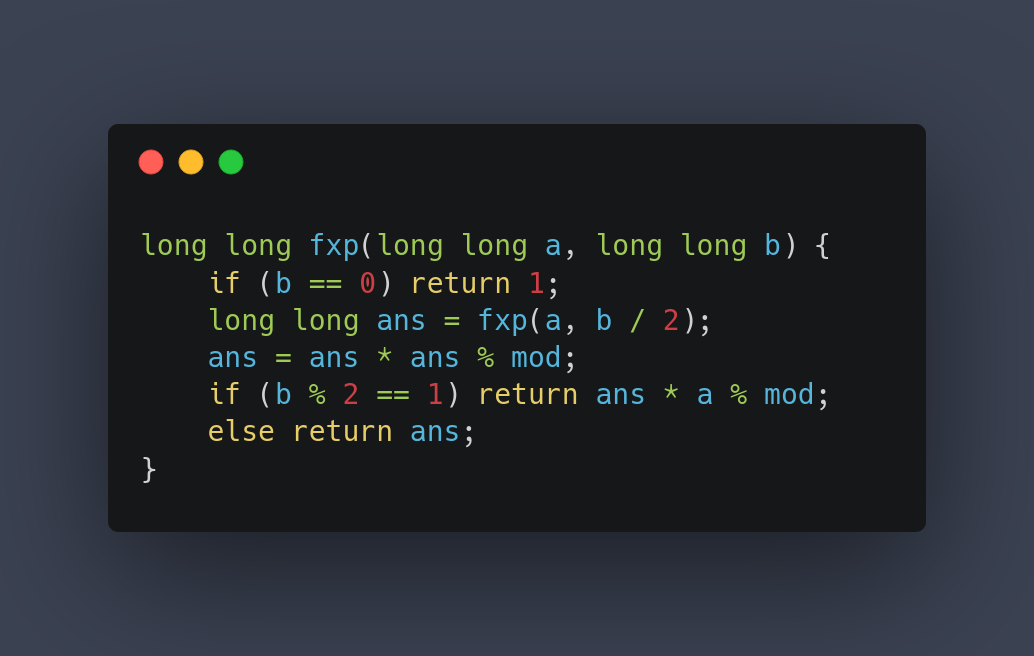
\includegraphics[scale=.25]{./img/fxp_rec.png}}
\end{frame}

\begin{frame}{Fast Modular Exponentation}{Implementazione iterativa}
    \makebox[\textwidth]{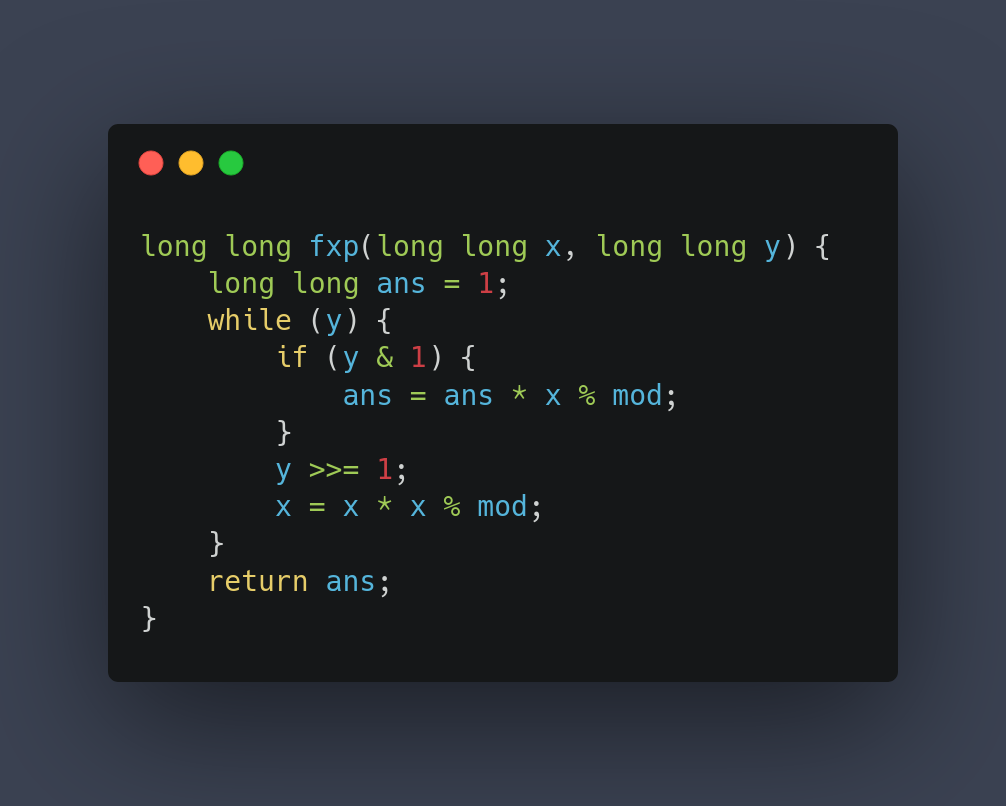
\includegraphics[scale=.25]{./img/fxp_iter.png}}
\end{frame}

\section{Teoria dei numeri}
\begin{frame}{Aritmetica modulare}
    Sia $m$ un intero positivo detto \textbf{modulo}. Gli interi $0,\dots,m-1$ prendono il nome di \textit{classi di resto} modulo $m$.
    \begin{itemize}
        \item due interi $a,b$ appartengono alla stessa classe di resto $r$ se entrambi danno resto $r$ nella divisione intera con $m$
        \item due interi appartenenti alla stessa classe di resto si dicono \textit{congrui} modulo $m$:
            $$a \equiv b \pmod m \iff m | (a-b)$$
        \pause
        \item in \textsc{C++}, l'operatore che associa un intero alla sua classe di resto\footnote{\textit{quasi} vero: \texttt{a \% mod} con \texttt{a} negativo restituisce un intero in $[m-1, 0]$} modulo \texttt{mod} \`e ``\texttt{\%}'', \texttt{12 \% 7 == 5}
    \end{itemize}
    \begin{block}{}
        Addizione, sottrazione e moltiplicazione funzionano normalmente anche sotto modulo (la divisione no!)
    \end{block}
\end{frame}

\begin{frame}{Numeri coprimi}{Phi di Eulero}
    Due interi $a, b$ si dicono \textit{coprimi}\footnote{o \textit{primi tra loro}} se il loro massimo comun divisore (gcd) \`e $1$.
    \begin{itemize}
        \item $1$ \`e coprimo con tutti
        \item $0$ non \`e coprimo con nessun intero $\geq 2$
    \end{itemize}
    \pause
    \vfill
    Sia $\phi(n)$\footnote{letto ``\textit{phi} di $n$''} il numero di interi coprimi con $n$ nel range $[1, n]$.
    \begin{block}{}
    \begin{itemize}
        \item $\phi(p) = p-1$ per ogni $p$ primo
        \item in generale, $\phi(p^k) = (p-1)p^{k-1} \ \forall k \in \mathbb{Z}_+$
        \item $\phi$ \`e una \textbf{funzione moltiplicativa}, ossia $\phi(a \cdot b) = \phi(a) \cdot \phi(b)$ per $a, b$ \textbf{coprimi}
    \end{itemize}
    \end{block}
    \pause
    \vfill
    Ok ma perch\`e dovrebbe interessarci?
\end{frame}

\begin{frame}{Teorema di Eulero}{Inversi modulari}
    \begin{block}{Teorema di Eulero}
        Per ogni coppia di interi $a,m$ coprimi,
        $$a^{\phi (m)} \equiv 1 \pmod m.$$
    \end{block}
    \pause
    In maniera equivalente,
    $$a \cdot (a^{\phi (m) - 1}) \equiv 1 \pmod m.$$
    \vfill
    Chiamiamo \textbf{inverso modulare} di $a$ un intero che moltiplicato con $a$ \`e congruo a $1 \pmod m$, $a^{\phi(m) - 1}$ \`e un inverso modulare di $a$.
    \pause
    \vfill
    Allora (se abbiamo un inverso) possiamo fare le divisioni!
    \vfill
    Sotto modulo $mod$ primo, invece che dividere per $x$ moltiplichiamo per $x^{p-2}$.
\end{frame}


\section{Combinatoria}
\begin{frame}{Permutazioni}
    \begin{exampleblock}{Permutazioni}
        Quante sono le permutazioni di $n$ elementi?
    \end{exampleblock}
    \vfill
    \pause
    Per la prima posizione abbiamo $n$ possibilit\`a, per la seconda $n-1$, per la terza $n-2$ e cos\`i via.
    \vfill
    \pause
    La risposta \`e quindi $n \cdot (n-1) \cdot (n-2) \cdot \dots \cdot 1$. Indichiamo questo prodotto come 
    $n!$\footnote{letto ``n fattoriale''}.
\end{frame}

\begin{frame}{Disposizioni}
    \begin{exampleblock}{Disposizioni}
        In quanti sono i possibili podi di una gara di $n$ partecipanti?
    \end{exampleblock}
    \vfill
    \pause
    Per la prima posizione abbiamo $n$ possibilit\`a, per la seconda $n-1$, per la terza $n-2$.\\
    \vfill
    \pause
    La risposta \`e quindi $n \cdot (n-1) \cdot (n-2)$.\\
    \vfill
    \pause
    In generale le disposizioni di $n$ elementi in $k$ posizioni sono \[\frac{n!}{(n-k)!}\]
\end{frame}

\begin{frame}{Combinazioni}
    \begin{exampleblock}{Combinazioni}
        In quanti possiamo scegliere $k$ elementi da un gruppo di $n$ elementi? (non importa l'ordine)
    \end{exampleblock}
    \pause
    Il problema \`e simile al precedente, ma ora non importa l'ordine degli elementi.
    Ci basta quindi dividere per $k!$.
    \pause
    La risposta \`e \[\frac{n!}{(n-k)! \cdot k!}\]
    \pause
Questa formula viene detta \textbf{Binomiale} e si indica come \[\binom{n}{k}\] \\
    \pause
    Nei problemi si chiede quasi sempre la risposta mod $10^9 + 7$. Di solito conviene precalcolare i fattoriali fino a $MAXN$ e i loro inversi modulari, per poi calcolare i binomiali all'occorrenza. 
\end{frame}

\begin{frame}{Implementazione}
    \makebox[\textwidth]{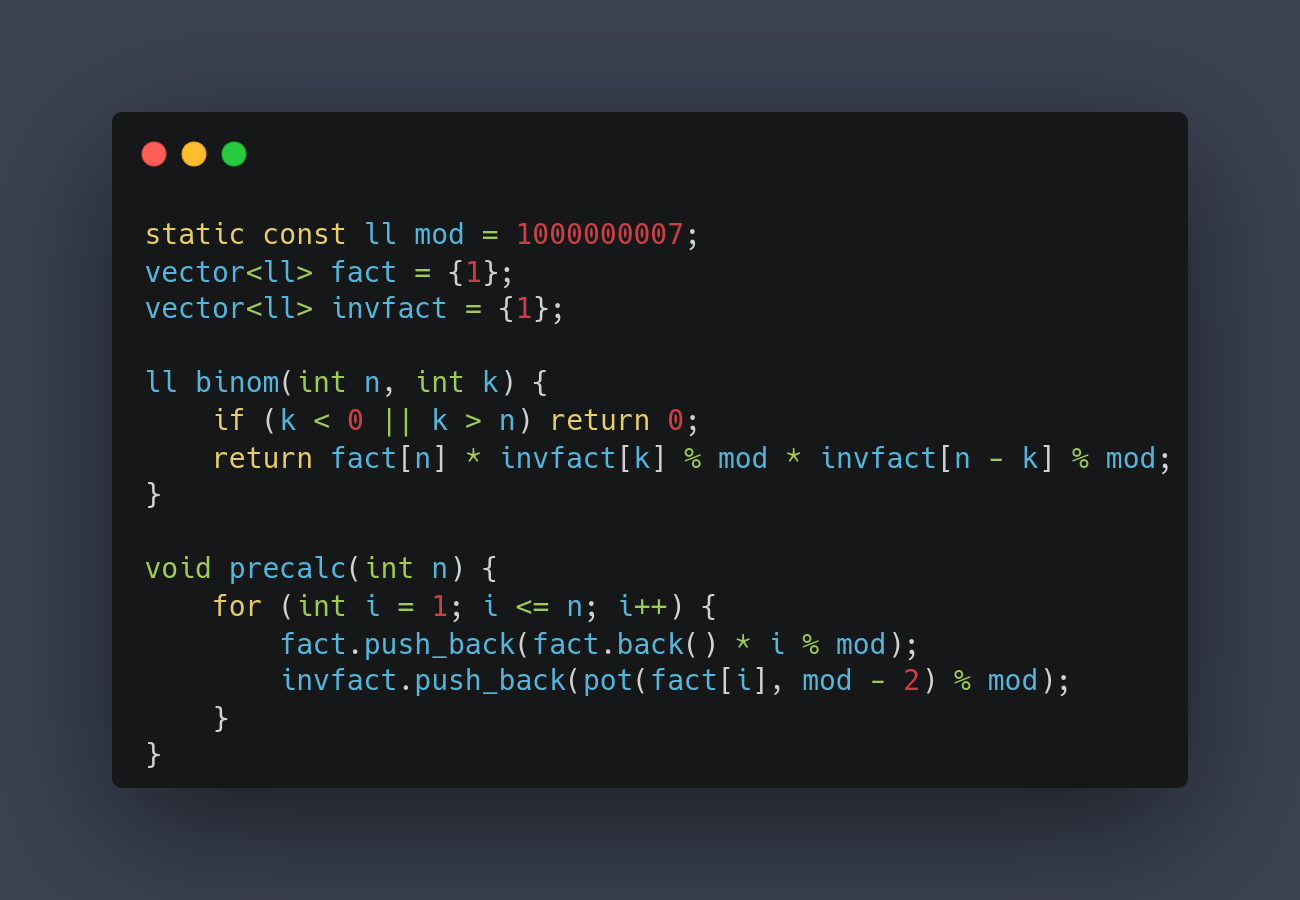
\includegraphics[scale=.25]{./img/comb.png}}
\end{frame}

\section{Rolling Hash}
\begin{frame}{String Matching}
    \begin{exampleblock}{String Matching}
        Date $N$ stringhe, controlla se ci sono due stringhe uguali.
    \end{exampleblock}
    \pause
    Risolvere il problema in modo naive richiederebbe $O(N^2)$, ma possiamo fare meglio.
    \pause
    \vfill
    Un modo semplice \`e utilizzare una \textbf{unordered\_set} o una \textbf{unordered\_map} e inserire le stringhe una alla volta, 
    controllando se la stringa che stiamo inserendo \`e gi\`a presente.
\end{frame}

\begin{frame}
    Ma esattamente come funzionano queste strutture dati?
    \vfill
    \pause
    Quello che ci interessa \`e che convertono una stringa in un numero, utilizzando una \textbf{funzione di hash}.
    La funzione di hash deve essere \textbf{deterministica}, ovvero dato lo stesso input, deve restituire sempre lo stesso output.\\
    \pause
    \vfill
    In questo modo se due stringhe hanno hash diversi, allora sono sicuramente diverse, 
    mentre se hanno hash uguali sono uguali \textbf{con una certa probabilit\`a}.\\
    \pause
    (Per evitare collisioni in alcuni problemi \`e necessario utilizzare pi\`u funzioni di hash).
\end{frame}

\begin{frame}
    Vediamo ora un esempio di funzione di hash, detto Rabin-Karp, che possiamo sfruttare per risolvere problemi anche pi\`u
    complessi.
    \pause
     \begin{exampleblock}{Algoritmo}
        Vediamo ogni stringa come un polinomio, ad esempio la stringa ``abc'' come $``a" \cdot x^2 + ``b" \cdot x + ``c"$ \\
        (dove ``a'' \`e il valore ascii del carattere 'a').\\
        \pause
        Scelti due interi $p$ e $m$, calcoliamo il valore del polinomio in $p$ modulo $m$, ovvero $(97 \cdot p^2 + 98 \cdot p + 99) \pmod m$.
    \end{exampleblock}
    \begin{alertblock}{Nota}
        \begin{itemize}
            \item $p$ e $m$ si scelgono primi\footnote{in realt\`a \`e sufficiente siano primi tra loro}\\
            \item $m$ deve essere abbastana grande (ad esempio $10^9 + 7$ o $10^9 + 9$).\\
            \item $p$ deve essere maggiore della dimensione dell'alfabeto (ad esempio un numero primo grande circa $200$-$300$).
        \end{itemize}
    \end{alertblock}
\end{frame}

\begin{frame}{Implementazione}
    \makebox[\textwidth]{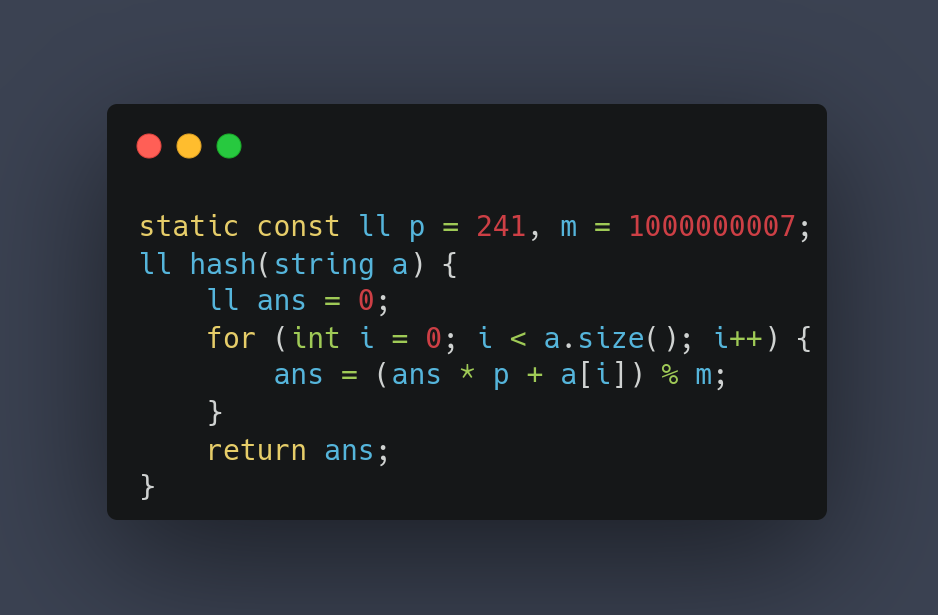
\includegraphics[scale=.35]{./img/hash.png}}
\end{frame}

\begin{frame}
    Perché questo algoritmo \`e utile?\\
    \pause
    Possiamo facilmente aggiornare l'hash di una stringa per calcolare quello di una stringa "simile", ad esempio:
    \pause
    \begin{itemize}
        \item $hash(s[a,b+1]) = hash(s[a,b]) \cdot p + s[b+1] \mod m$.
        \item $hash(s[a+1,b]) = (hash(s[a,b]) - s[a] \cdot p^{b-a}) \mod m$.
        \item $hash(s[k+1,b]) = hash(s[a,b]) - (hash(s[a,k]) \cdot p^{b-k}) \mod m$.
    \end{itemize}
    \pause
    Proprio per questo motivo questo algoritmo \`e anche chiamato \textbf{Rolling Hash}.
    Questo \`e molto utile per risolvere numerosi problemi su stringhe.
\end{frame}

\begin{frame}
    \begin{exampleblock}{Pattern Matching}
        Date due stringhe $s$ e $t$, conta il numero di occorrenze di $t$ in $s$.
        \vfill
        \small{\underline{\url{https://cses.fi/problemset/task/1753/}}}
    \end{exampleblock}
    \pause
    Esistono numerosi algoritmi per risolvere questo problema, come Z-Algorithm, KMP, etc...\\
    \pause
    Possiamo facilmente risolverlo con Rolling Hash:
    \begin{itemize}
        \item Siano $N$ la lunghezza di $s$ e $M$ la lunghezza di $t$.
        \item Calcoliamo l'hash di $t$ e chaimiamolo $target$.
        \item Calcoliamo l'hash dei primi $M$ caratteri di $s$ e chiamiamolo $curr$.
        \item Aggiorniamo $curr$ aggiungiendo il carattere successivo di $s$ e togliendo il primo.
        \item Ogni volta che $curr$ \`e uguale a $target$ abbiamo trovato un match (molto probabilmente).
    \end{itemize}
\end{frame}

\section{Problemi}
\begin{frame}{Problemi}
    \small{\underline{\url{https://cses.fi/problemset/task/1095}}}
    \small{\underline{\url{https://cses.fi/problemset/task/1712}}}
    \small{\underline{\url{https://training.olinfo.it/\#/task/ois_scount/statement}}}
    \small{\underline{\url{https://training.olinfo.it/\#/task/ois_walker/statement}}}
    \small{\underline{\url{https://training.olinfo.it/\#/task/ois_casino/statement}}}
    \small{\underline{\url{https://training.olinfo.it/\#/task/itoi_morse/statement}}}
    \small{\underline{\url{https://training.olinfo.it/\#/task/unimi_glitch/statement}}}
\end{frame}

\end{document}
